\chapter{Reproduksi dan Lingkungan}\label{ch:g8:reproduction-and-environment}

Mengapa paduan suara katak bermula pada bulan Mei dan bukan bulan
November? Mengapa sebuah tahun beech yang baik memenuhi hutannya
dengan \omterm{prop:g2:from-seed-to-plant:cycle}{kecambah}, dan sebuah bulan Juni yang dingin dan basah
mengosongkan kolam musim semi berikutnya dari katak kecil? Bab yang
lalu membangun mekanisme generasi berikutnya; bab ini menancapkannya
ke dalam dunianya: reproduksi diatur waktunya, dibekali --- dan
dibatasi --- oleh \omterm{def:g6:exploring-our-environment:components}{lingkungannya}.

\section{Diatur waktunya oleh musim}

\begin{proposition}[Pembiakan mengikuti penanggalan kelimpahan]\label{prop:g8:reproduction-and-environment:timing}
\omterm{def:g5:biodiversity:species}{Spesies} mengatur waktu reproduksinya sehingga \emph{anaknya} tiba
ketika \omterm{def:g6:exploring-our-environment:conditions}{kondisi} dan makanannya akan melayaninya
(\cref{prop:g6:life-through-seasons:conditions}):
\begin{itemize}
  \item gelatik biru bertelur sehingga anaknya menetas pada puncak
        \omterm{ex:g2:animals-grow-up:butterfly}{ulat} musim semi (rantai pohon ek pada
        \cref{ex:g3:food-chains:three}, yang diatur waktunya sampai ke
        harinya);
  \item katak mengeluarkan \omterm{def:g2:animals-grow-up:born}{telurnya} di kolam yang menghangat,
        sehingga \omterm{ex:g2:animals-grow-up:frog}{berudunya} memperoleh satu musim panas untuk tumbuh
        sebelum musim dingin;
  \item \omterm{def:g1:plants-around-us:plant}{tumbuhan} berbunga menurut musim penyerbuknya lalu memasakkan
        \omterm{def:g2:from-seed-to-plant:seed}{bijinya} menurut penanggalan \omterm{def:g6:how-plants-spread:dispersal}{penyebarannya}
        (\cref{pb:g6:life-through-seasons:1});
  \item lenguhan musim gugur sang rusa \omterm{def:g4:animal-reproduction:sexual}{jantan} menetapkan \omterm{def:g2:born-grow-die:cycle}{kelahirannya}
        pada \emph{musim semi} berikutnya --- masa kandungannya sudah
        diperhitungkan.
\end{itemize}
Isyarat yang memulai permesinannya adalah isyarat \omterm{def:g6:exploring-our-environment:components}{lingkungannya}
sendiri: terutama hari yang memanjang, kehangatan, hujan.
\end{proposition}
\admitted

\begin{omfigure}
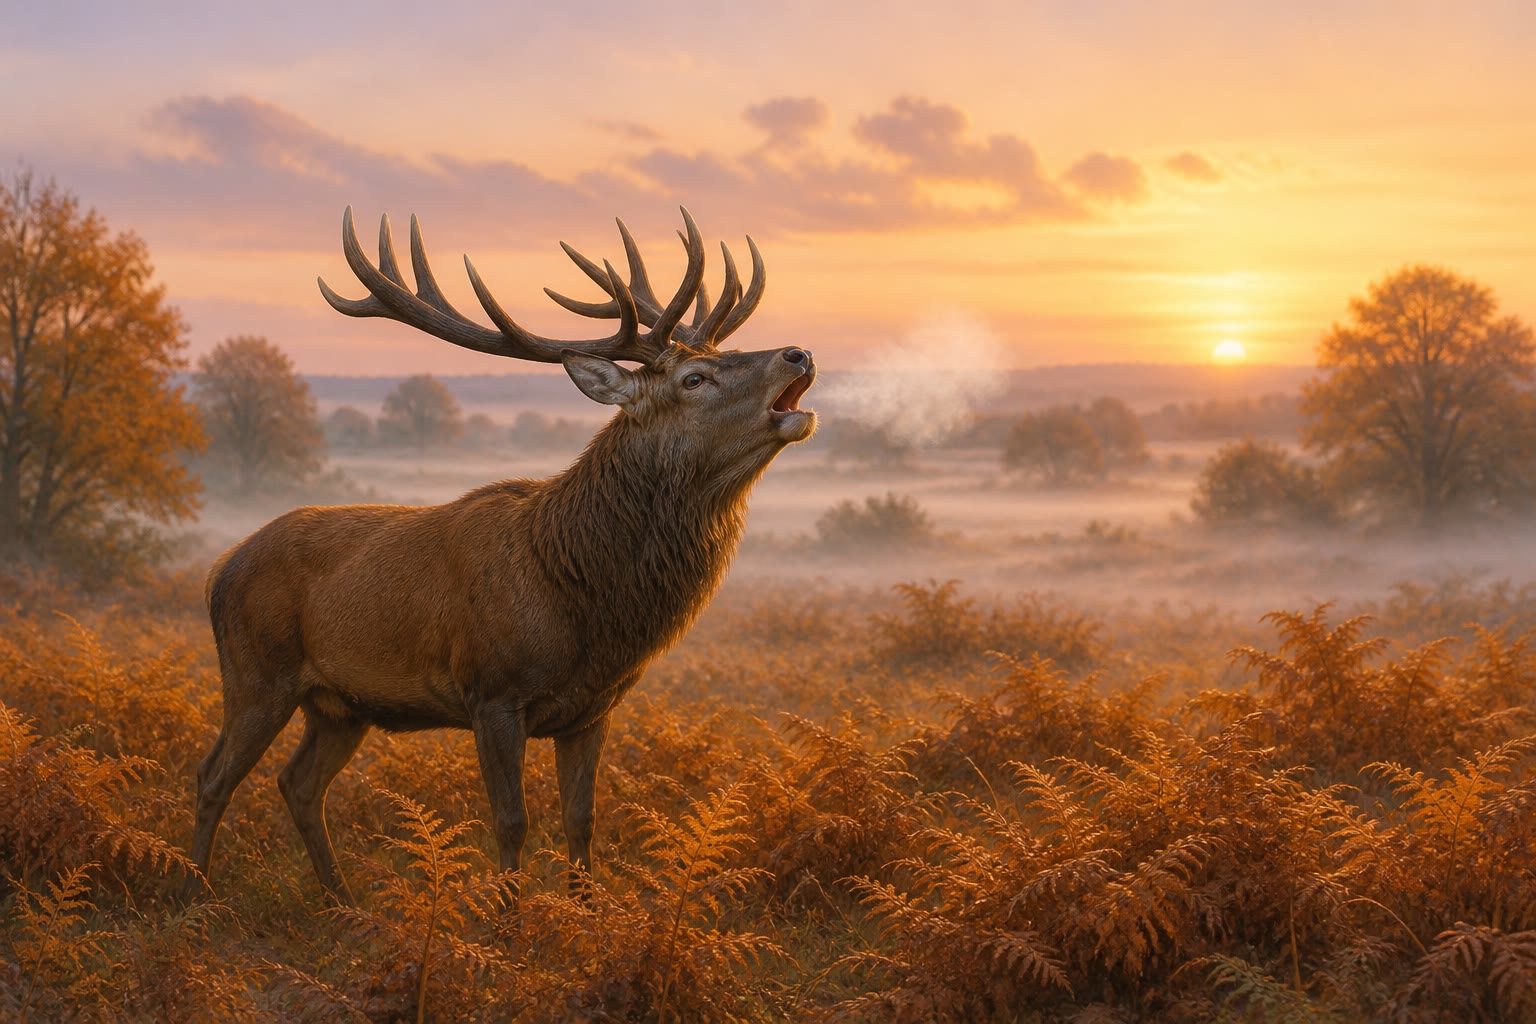
\includegraphics[width=0.6\linewidth]{images/book1/ai/g8-repro-stag.jpg}

{\small Lenguhan musim gugur, hitung-hitungan musim semi: pengaturan
waktu sang rusa \omterm{def:g4:animal-reproduction:sexual}{jantan} memperhitungkan masa kandungannya.}
\end{omfigure}

\begin{omfigure}
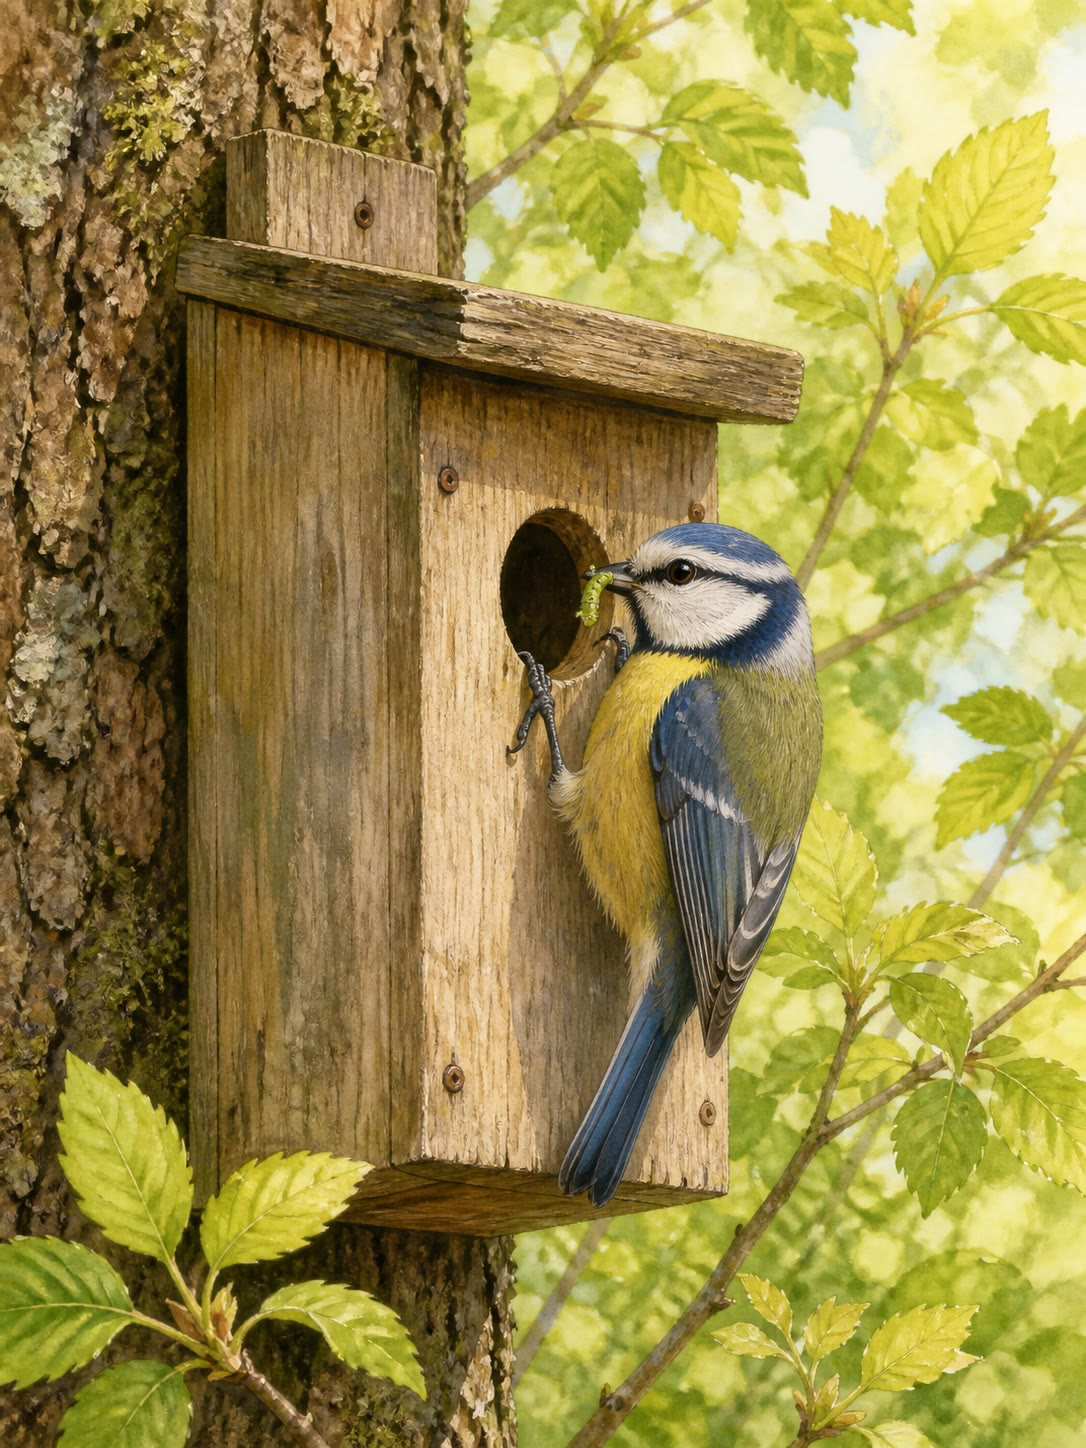
\includegraphics[width=0.46\linewidth]{images/book1/ai/g8-env-nestbox.jpg}

{\small Mutu \omterm{def:g2:where-animals-live:habitat}{habitat}, yang diantarkan: seekor gelatik biru dan \omterm{ex:g2:animals-grow-up:butterfly}{ulat}
yang menjadi acuan waktu kelompok \omterm{def:g2:animals-grow-up:born}{telurnya}.}
\end{omfigure}

\begin{example}[Anak domba dalam ruangan]\label{ex:g8:reproduction-and-environment:lambs}
Peternak domba memanfaatkan isyaratnya secara langsung: domba \omterm{def:g4:animal-reproduction:sexual}{betina}
masuk ke keadaan siap \omterm{prop:g4:animal-reproduction:where}{kawin} ketika harinya \emph{memendek}; kalau
dipelihara di bawah \omterm{def:g6:exploring-our-environment:conditions}{cahaya} buatan yang dipanjangkan lalu dipendekkan,
sekawanan domba dapat dibuat beranak untuk pasar awal yang
menguntungkan. Permesinannya membaca \omterm{def:g6:exploring-our-environment:conditions}{cahaya}, bukan penanggalan ---
ubahlah \omterm{def:g6:exploring-our-environment:conditions}{cahayanya} dan penanggalannya mengikuti. Isyarat yang diketahui
adalah sebuah tuas.
\end{example}

\section{Dibekali oleh habitatnya}

\begin{proposition}[Reproduksi dibayar dengan materi]\label{prop:g8:reproduction-and-environment:cost}
\omterm{def:g2:animals-grow-up:born}{Telur}, \omterm{def:g2:animals-grow-up:born}{susu}, nektar, \omterm{def:g2:from-seed-to-plant:seed}{biji} dan ranggah semuanya adalah \emph{produksi}
dalam pengertian
\cref{def:g6:matter-from-food:production} --- \omterm{def:g6:plants-are-producers:matter}{materi organik} yang
harus diperoleh induknya lebih dahulu. Karena itu kekayaan \omterm{def:g2:where-animals-live:habitat}{habitatnya}
menetapkan anggarannya:
\begin{itemize}
  \item seekor ayam yang cukup makan bertelur setiap hari; yang
        kelaparan berhenti --- pembukuan pada
        \cref{pb:g6:matter-from-food:1} yang berimbang pada baris
        \omterm{def:g2:animals-grow-up:born}{telurnya};
  \item pohon beech berbuah besar-besaran hanya pada ``tahun panen
        raya'' yang menyusul musim tumbuh yang baik --- panen \omterm{def:g2:from-seed-to-plant:seed}{bijinya}
        adalah musim panas yang ditabung
        (\cref{ex:g6:plants-are-producers:pantry});
  \item tahun yang sulit menipiskan kelompok \omterm{def:g2:animals-grow-up:born}{telurnya}: banyak \omterm{prop:g3:sorting-living-things:groups}{burung}
        bertelur lebih sedikit, atau tidak sama sekali, ketika
        mangsanya kurang.
\end{itemize}
\end{proposition}
\admitted

\begin{example}[Menghitung kelompok telur gelatiknya]\label{ex:g8:reproduction-and-environment:clutch}
Kajian kotak sarang memperlihatkan kelompok \omterm{def:g2:animals-grow-up:born}{telur} gelatik biru
mengikuti persediaan \omterm{ex:g2:animals-grow-up:butterfly}{ulatnya}: hutan ek yang kaya, sepuluh \omterm{def:g2:animals-grow-up:born}{telur} atau
lebih; kebun yang miskin, enam atau tujuh. \omterm{prop:g3:sorting-living-things:groups}{Burungnya} tidak memutuskan
hal ini dengan sebuah pembukuan --- keadaan tubuhnya, yang dibangun
dari makanan \omterm{def:g2:where-animals-live:habitat}{habitatnya}, menetapkan berapa banyak yang dapat
dibekalinya. Besarnya kelompok \omterm{def:g2:animals-grow-up:born}{telur} adalah mutu \omterm{def:g2:where-animals-live:habitat}{habitat}, yang
tertulis dalam bentuk \omterm{def:g2:animals-grow-up:born}{telur}.
\end{example}

\section{Dibatasi oleh dunianya: populasi}

\begin{definition}[Populasi]\label{def:g8:reproduction-and-environment:population}
Suatu \emph{populasi}\index{populasi} adalah semua individu satu
\omterm{def:g5:biodiversity:species}{spesies} yang hidup di satu tempat --- katak di kolamnya, pohon beech di
hutannya. Reproduksi menambahnya; kematian dan kepergian
menguranginya; \omterm{def:g6:exploring-our-environment:components}{lingkungannya} menetapkan langit-langitnya.
\end{definition}

\begin{proposition}[Mengapa populasi tidak meledak]\label{prop:g8:reproduction-and-environment:limits}
Setiap \omterm{def:g5:biodiversity:species}{spesies} menghasilkan berlebih --- ribuan \omterm{def:g2:animals-grow-up:born}{telur} per pasangan
katak, ribuan \omterm{def:g2:from-seed-to-plant:seed}{biji} per pohon beech
(\cref{prop:g4:animal-reproduction:strategies}) --- namun kolamnya
tidak padat oleh katak. Kelebihannya dibelanjakan melawan penahan
\omterm{def:g6:exploring-our-environment:components}{lingkungannya}:
\begin{itemize}
  \item \emph{pemangsaan} --- kuntul dan larva capung pada
        \cref{ex:g4:animal-reproduction:pondcount};
  \item \emph{makanan dan ruang} --- \omterm{ex:g2:animals-grow-up:butterfly}{ulat}, lubang sarang, dan petak
        \omterm{def:g6:exploring-our-environment:conditions}{cahaya} di lantai hutannya hanya sekian banyaknya;
  \item \emph{\omterm{def:g6:exploring-our-environment:conditions}{kondisi}} --- embun beku yang terlambat pada \omterm{def:g3:flowers-fruits-seeds:parts}{bunganya}
        (\cref{exo:g3:flowers-fruits-seeds:9}), kemarau pada kolam
        \omterm{ex:g2:animals-grow-up:frog}{berudunya} yang menyusut.
\end{itemize}
Rata-rata, di dalam sebuah \omterm{def:g2:where-animals-live:habitat}{habitat} yang mantap, tiap pasangan
menggantikan dirinya sendiri --- keseimbangan pada
\cref{prop:g5:food-webs:balance}, yang dilihat dari sisi induknya.
\end{proposition}
\admitted

\begin{example}[Dua musim semi di kolamnya]\label{ex:g8:reproduction-and-environment:twosprings}
Musim semi 1, lunak dan basah: airnya tinggi, \omterm{prop:g3:sorting-living-things:groups}{serangganya} datang awal
--- ribuan \omterm{def:g2:animals-grow-up:born}{telur}, ratusan katak kecil, \omterm{def:g8:reproduction-and-environment:population}{populasinya} menanjak. Musim
semi 2, sebuah kemarau: kolamnya menyusut menjadi genangan, \omterm{ex:g2:animals-grow-up:frog}{berudunya}
berdesakan, \omterm{def:g7:what-is-respiration:respiration}{oksigennya} turun
(\cref{prop:g7:oxygen-in-the-water:drains}), kuntulnya berpesta atas
gerombolan yang memekat --- segelintir katak kecil. Katak yang sama,
mekanisme yang sama, dua putusan: \omterm{def:g6:exploring-our-environment:components}{lingkungannya} menandatangani balik
setiap generasinya.
\end{example}

\begin{remark}[Manusia menggeser penahannya]\label{rem:g8:reproduction-and-environment:humans}
Kebanyakan pengaruh manusia atas satwa liar berjalan lewat penahan
ini, bukan lewat mekanisme intinya: kolam yang dikeringkan dan pagar
tanaman yang dibongkar menyingkirkan \omterm{def:g2:where-animals-live:habitat}{habitat} pembiakannya
(\cref{prop:g2:where-animals-live:loss}); pestisida mengosongkan
puncak \omterm{ex:g2:animals-grow-up:butterfly}{ulat} yang menjadi acuan waktu gelatiknya; kotak sarang di kebun
dan padang rumput basah yang dipulihkan pada
\cref{ex:g5:biodiversity:storks} menambahkan langit-langitnya kembali.
Melindungi sebuah \omterm{def:g5:biodiversity:species}{spesies} dalam praktiknya berarti melindungi
\omterm{def:g6:exploring-our-environment:components}{lingkungan} tempat reproduksinya ditancapkan --- isyarat, anggaran dan
penahannya sekaligus.
\end{remark}

\begin{method}[Mengaudit sebuah perubahan populasi]\label{met:g8:reproduction-and-environment:audit}
Ketika sebuah \omterm{def:g8:reproduction-and-environment:population}{populasi} naik atau turun, auditlah secara berurutan:
\begin{enumerate}
  \item \emph{pengaturan waktunya}: apakah isyaratnya dan puncak
        sumber dayanya masih berimpit? (musim semi yang datang terlalu
        awal dapat menelantarkan anaknya sesudah \omterm{ex:g2:animals-grow-up:butterfly}{ulatnya} lewat);
  \item \emph{anggarannya}: apa yang dibiarkan \omterm{def:g2:where-animals-live:habitat}{habitat} musim itu untuk
        dibekalkan induknya?
  \item \emph{penahannya}: mana yang berubah --- pemangsa, makanan,
        ruang, \omterm{def:g6:exploring-our-environment:conditions}{kondisi}?
  \item \emph{\omterm{def:g2:where-animals-live:habitat}{habitatnya}}: apakah lahan pembiakannya sendiri bertambah
        atau hilang?
\end{enumerate}
\end{method}

\section{Latihan}

\begin{exercise}[$\star$]\label{exo:g8:reproduction-and-environment:1}
Mengapa gelatik biru bertelur pada waktu ia bertelur? Sebutkan
aturannya dan isyaratnya.
\end{exercise}

\begin{exercise}[$\star$]\label{exo:g8:reproduction-and-environment:2}
Apa yang dicapai pengaturan waktu musim gugur sang rusa \omterm{def:g4:animal-reproduction:sexual}{jantan}, dan
apa yang harus diperhitungkan?
\end{exercise}

\begin{exercise}[$\star$]\label{exo:g8:reproduction-and-environment:3}
Mengapa reproduksi ``dibayar dengan materi''? Berikan tiga
pembayarannya dari
\cref{prop:g8:reproduction-and-environment:cost}.
\end{exercise}

\begin{exercise}[$\star$]\label{exo:g8:reproduction-and-environment:4}
Apa itu \omterm{def:g8:reproduction-and-environment:population}{populasi}? Apa yang menambah, apa yang mengurangi, apa yang
menetapkan langit-langitnya?
\end{exercise}

\begin{exercise}[$\star$]\label{exo:g8:reproduction-and-environment:5}
Sebutkan ketiga penahan yang membelanjakan kelebihan kataknya.
\end{exercise}

\begin{exercise}[$\star$]\label{exo:g8:reproduction-and-environment:6}
Apa yang dilaporkan kelompok \omterm{def:g2:animals-grow-up:born}{telur} gelatik sepuluh butir dibandingkan
enam butir, dan tentang apa?
\end{exercise}

\begin{exercise}[$\star\star$]\label{exo:g8:reproduction-and-environment:7}
Jelaskan kiat \omterm{def:g6:exploring-our-environment:conditions}{cahaya} para peternak dombanya, dan apa yang
dibuktikannya tentang isyarat.
\end{exercise}

\begin{exercise}[$\star\star$]\label{exo:g8:reproduction-and-environment:8}
Ceritakan kembali \cref{ex:g8:reproduction-and-environment:twosprings}
sebagai keempat pertanyaan
\cref{met:g8:reproduction-and-environment:audit}, yang dijawab untuk
musim semi 2.
\end{exercise}

\begin{exercise}[$\star\star$]\label{exo:g8:reproduction-and-environment:9}
Sebuah iklim yang menghangat mendatangkan \omterm{ex:g2:animals-grow-up:butterfly}{ulat} pohon ek dua minggu
lebih awal, tetapi isyarat panjang hari gelatiknya tidak berubah.
Ramalkan ketidakcocokannya dan baris auditnya.
\end{exercise}

\begin{exercise}[$\star\star$]\label{exo:g8:reproduction-and-environment:10}
``Jutaan \omterm{def:g2:animals-grow-up:born}{telur} \omterm{prop:g3:sorting-living-things:groups}{ikan} kod tidak terbuang --- keduanya dibelanjakan.''
Belalah kalimat itu dengan
\cref{prop:g8:reproduction-and-environment:limits}.
\end{exercise}

\begin{exercise}[$\star\star$]\label{exo:g8:reproduction-and-environment:11}
Penahan yang mana yang digeser tiap tindakan manusia ini: mengeringkan
sebuah rawa; menggantungkan kotak sarang; menyemprot kebun \omterm{prop:g3:flowers-fruits-seeds:transform}{buahnya}
terhadap \omterm{ex:g2:animals-grow-up:butterfly}{ulat} pada bulan Mei; memulihkan sebuah padang rumput basah?
\end{exercise}

\begin{exercise}[$\star\star\star$]\label{exo:g8:reproduction-and-environment:12}
Hubungkan tiga bab dalam satu alinea: garis siasatnya
(\cref{prop:g4:animal-reproduction:strategies}), kehilangan pada
piramidanya (\cref{ex:g6:matter-from-food:pyramid}), dan penahan bab
ini --- sebagai satu penjelasan tentang mengapa kolamnya tidak padat
oleh katak.
\end{exercise}

\section{Soal: Pembukuan Kotak Sarang}

\begin{problem}[{Soal akhir pekan --- sepuluh tahun perjalanan gelatik
biru, yang diaudit kotak demi kotak}]\label{pb:g8:reproduction-and-environment:1}
Sebuah sekolah memantau dua puluh kotak sarang selama sepuluh tahun:
tanggal bertelurnya, besar kelompok \omterm{def:g2:animals-grow-up:born}{telurnya}, jumlah anak yang berhasil
terbang tiap kotaknya --- di samping catatan cuacanya dan buku harian
penjaga halamannya.

\medskip\noindent\textbf{Bagian I --- Membaca tahun yang
biasa.}
\begin{enumerate}
  \item Tahun 1--4: bertelur pada akhir bulan April, kelompok \omterm{def:g2:animals-grow-up:born}{telurnya}
        delapan sampai sepuluh butir, kebanyakan \omterm{def:g2:animals-grow-up:born}{telurnya} berhasil
        terbang. Sebutkan isyarat yang menetapkan akhir April itu, dan
        puncak yang menjadi sasaran pengaturan waktunya.
  \item Kelompok \omterm{def:g2:animals-grow-up:born}{telur} tahun 3 berjumlah satu atau dua butir lebih
        besar sesudah bulan Mei tahun 2 yang hangat dan kaya \omterm{ex:g2:animals-grow-up:butterfly}{ulat} ---
        induknya melewati musim dinginnya dengan baik. Proposisi yang
        mana yang digambarkan hubungan itu?
  \item Bahkan pada tahun yang baik, kira-kira seperlima \omterm{def:g2:animals-grow-up:born}{telurnya} tidak
        pernah berhasil terbang. Daftarkan penahan yang mungkin
        bertanggung jawab, dari
        \cref{prop:g8:reproduction-and-environment:limits}.
  \item Mengapa sekolahnya mencatat cuaca dan pekerjaan halamannya di
        samping \omterm{def:g2:animals-grow-up:born}{telurnya}? (Jawablah dengan keempat pertanyaan
        auditnya.)
\end{enumerate}

\medskip\noindent\textbf{Bagian II --- Keganjilannya.}
\begin{enumerate}[resume]
  \item Tahun 5: bulan Maret yang luar biasa hangat mengeluarkan
        \omterm{ex:g2:animals-grow-up:butterfly}{ulatnya} dua minggu lebih awal; tanggal bertelurnya nyaris
        tidak bergeser. Ramalkan keberhasilan terbang tahun 5, lalu
        sebutkan baris kegagalan pada auditnya.
  \item Tahun 6: buku harian penjaga halamannya mencatat dahan mati
        pohon ek yang tua disingkirkan dan jalur padang rumputnya
        dipangkas tiap bulan. Keberhasilan terbangnya turun walaupun
        cuacanya ramah. Baris audit mana yang ditunjuk buku hariannya?
  \item Tahun 7: sepasang alap-alap menetap. Kelompok \omterm{def:g2:animals-grow-up:born}{telurnya} tidak
        berubah, tetapi jumlah anak yang berhasil terbang melorot.
        Penahan yang mana yang bergeser, dan mengapa baris
        \emph{kelompok \omterm{def:g2:animals-grow-up:born}{telurnya}} tidak ikut bergeser?
  \item Tahun 8: kotaknya dilipatduakan menjadi empat puluh; jumlah
        seluruh anak yang berhasil terbang naik, tetapi keberhasilan
        \emph{per kotak} bertahan tetap. Langit-langit apa yang
        dinaikkan kotak barunya, dan langit-langit mana yang
        dibiarkannya tidak tersentuh?
\end{enumerate}

\medskip\noindent\textbf{Bagian III --- Laporannya.}
\begin{enumerate}[resume]
  \item Tuliskan kalimat rangkuman sepuluh tahunnya yang menghubungkan
        besar kelompok \omterm{def:g2:animals-grow-up:born}{telur} dengan mutu \omterm{def:g2:where-animals-live:habitat}{habitat}, dengan mengutip
        \cref{ex:g8:reproduction-and-environment:clutch}.
  \item Kotanya mengusulkan menebang barisan pohon eknya untuk sebuah
        tempat parkir, dengan ``ganti rugi'' berupa lima puluh kotak
        sarang tambahan. Auditlah tawarannya: di antara isyarat,
        anggaran, penahan dan \omterm{def:g2:where-animals-live:habitat}{habitat}, mana yang digantikan kotaknya,
        dan mana yang hanya disediakan pohon eknya?
  \item Sarankan dua tindakan halaman untuk tahun ke-11, masing-masing
        terikat pada baris auditnya.
  \item Tutuplah dengan pelajaran moral bab ini dalam satu kalimat:
        selain dua induk, apa lagi yang dibutuhkan setiap anak yang
        akan terbang?
\end{enumerate}
\end{problem}
